\documentclass[aspectratio=169,10pt]{beamer}

\usetheme{metropolis}
\usepackage{appendixnumberbeamer}
%\usepackage[utf8x]{inputenc} % but utf8 would be better
\usepackage[english]{babel}
\usepackage{booktabs}
\usepackage[scale=2]{ccicons}
\usepackage{bbm}

\usepackage{pgfplots}
\usepgfplotslibrary{dateplot}
\setbeamertemplate{caption}{\raggedright\insertcaption\par}% remove caption

%\usepackage{xspace}
\newcommand{\themename}{\textbf{\textsc{metropolis}}\xspace}
%%%%%%%%%%%% bloque teorema
%\setbeamercolor{block body}{bg=mDarkTeal!30}
%\setbeamercolor{block title}{bg=mDarkTeal,fg=black!2}
%cambiar fuente de letra equaciones
\usefonttheme[onlymath]{serif}




%\definecolor{niceRed}{HTML}{d20000}
% \definecolor{niceOrange}{HTML}{f59a23}
% \definecolor{niceGreen}{HTML}{7ec636}
%\definecolor{niceBlue}{HTML}{007aff}
\definecolor{mpigreen}{HTML}{007977}

\setbeamercolor{frametitle}{bg=mpigreen}
% para justificar
\usepackage{lipsum}
\usepackage{ragged2e}
\newcommand{\jus}{\justifying}
\apptocmd{\frame}{}{\justifying}{}
\apptocmd{\block}{}{\justifying}{}
\apptocmd{\column}{}{\justifying}{}
\DeclareMathOperator{\modi}{mod}
\DeclareMathOperator{\e}{e}
\DeclareMathOperator{\arf}{argmax}

\usepackage{amsmath, bm}
%\usepackage{mathspec}
\usepackage{mathrsfs}
\usepackage{dsfont}
\usepackage{bbold}
\usepackage{mathabx}%for widebar
\def\kay{\ensuremath{\mscrk}}

% para tablas 
\usepackage{booktabs}

\usepackage{amssymb}
\usepackage{amsfonts}


\usepackage{graphicx}  % Required for including images
\usepackage{tabularx}
%\usepackage{tikz}
\usepackage{float}
\usepackage{color}
\usepackage{mathtools}

\usepackage{array}
\usepackage{multirow}
\usepackage{wrapfig}
\usepackage{colortbl}
\usepackage{pdflscape}
\usepackage{xcolor}
\usepackage{longtable}
\usepackage{multirow}
\usepackage{wrapfig}
\usepackage{colortbl}
\usepackage{pdflscape}
\usepackage{tabu}
\usepackage{threeparttable}
\usepackage{threeparttablex}
\usepackage[normalem]{ulem}
\usepackage{makecell}
\usepackage{xcolor}
\usepackage{subcaption}
\captionsetup[sub]{labelfont=bf,textfont=bf}

%para break 2 frames
 %\renewcommand\frame[1][]{\oldframe[allowframebreaks,#1]}
%\let\oldframe\frame
%\renewcommand\frame[1][allowframebreaks]{\oldframe[#1]}

% quitar linea de progreso
%\metroset{numbering=fraction}
%\metroset{progressbar=frametitle}
%\metroset{background=dark}

%\setbeamercolor{palette primary}{bg=white,fg=white}
%\setbeamercolor{background canvas}{parent=palette primary}
%\setbeamercolor{normal text}{fg=white}
%\setbeamercolor{progress bar}{use=palette primary,fg=red,bg=red}
%----------------------------------------------------------------------------------------



\title{ Identifying Departures from the Fully Developed Speckle Hypothesis in Intensity SAR Data with Non-Parametric Estimation of the Entropy}


\author{Janeth Alpala \and Abraão D.~C.~Nascimento \and \textbf{\underline{Alejandro C.~Frery}}}
\date{\textcolor{black}{}}
%\institute{\textcolor{black}{Programa de Pos-graduação em Estatística da UFPE})}
% \institute{ Programa de Pos-graduação em Estatística da UFPE}
 
\titlegraphic{
\begin{picture}(0,0)
\put(\dimexpr\paperwidth-1.4cm,-120){\makebox(0,0)[rt]{
\includegraphics[width=6.0cm]{./Figures/Migars_600x450.png}}}
\put(20,-170){\makebox(0,0)[lt]{
\includegraphics[width=2.5cm]{./Figures/ufpe.png}}}
\put(120,-171){\makebox(0,0)[lt]{
\includegraphics[width=3.5cm]{./Figures/vic.png}}}
\end{picture}
}

\begin{document}

\maketitle
%----------------------------------------------------------------------------------------
\begin{frame}{Outline}
  \setbeamertemplate{section in toc}[sections numbered]
  \tableofcontents[hideallsubsections]
\end{frame}
\section{Context and Problem Statement}
%----------------------------------------------------------------------------------------
\begin{frame} \frametitle{\large{Context}}\vspace{-0.3cm}	

 \justifying
\begin{columns}[T,onlytextwidth]
    \begin{column}{.55\textwidth}
			\begin{alertblock}{Fully Developed Speckle (FDS)}\justifying
			\vspace{0.4cm}	
Homogeneous areas in SAR images are characterized by the lack of dominant scatterers, and the surface can be considered stationary.
This is the case of the \textbf{fully developed hypothesis for the speckle}.

%The speckle noise follows a well-defined statistical distribution, typically modeled as a Gamma distribution. 
		 \vspace{0.4cm}	
	\end{alertblock}
	\begin{alertblock}{Optimal model}\justifying
	\vspace{0.2cm}	
		The \(\mathcal{G}^0\) distribution is a suitable model for SAR intensity data. %because it describes  areas with different degrees of texture. 
		It includes the \textbf{Gamma law} as a limit case that results in the presence of fully developed speckle.


	\end{alertblock}
		
    \end{column}
    \begin{column}{.40\textwidth}\vspace{-0.8cm}
		     \begin{block}{} 
		\justifying
				\begin{figure}[H]
    \centering
    \subfloat[\scriptsize{FDS (agricultural area)}]{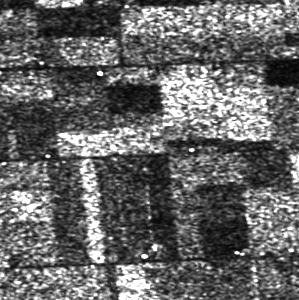
\includegraphics[width=30mm]{./Figures/Flevoland_300} }\hfill
    \subfloat[\scriptsize{Heterogeneous clutter (urban area)}]{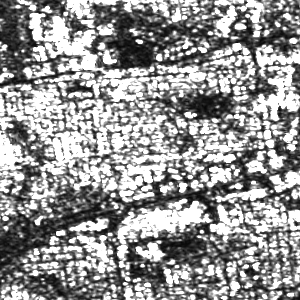
\includegraphics[width=30mm]{./Figures/Urban_Ottawa} }\vspace{-0.4cm}
    \caption*{SAR images.}
    \label{fig:real_SAR_Images_coe}
\end{figure}
\end{block}\vspace{2.8cm}
    \end{column}
\end{columns}\vspace{0.2cm}
%\metroset{block=fill}
      %\begin{exampleblock}{Objetive}
       
      %\end{exampleblock}

\end{frame} 
%----------------------------------------------------------------------------------------
\begin{frame} \frametitle{\large{Problem and Proposal}}\vspace{0.4cm}	

 \justifying
\begin{columns}[T,onlytextwidth]
    \begin{column}{.8\textwidth}
			\begin{exampleblock}{}\justifying
Selecting the optimal statistical model to characterize speckle in SAR data presents challenges. 
\pause
\begin{itemize}
    \item Opting for the \textbf{Gamma law }with $\mathcal{G}^0$ data:
    \begin{itemize}
        \item Loss of the information about the number of scatterers.
    \end{itemize}
		\pause
    \item \textbf{Applying $\mathcal{G}^0$} under fully developed speckle:
    \begin{itemize}
        \item Tricky maximum likelihood estimation:
       Increased bias, flat likelihood, and numerical optimization may not
converge.
        
    \end{itemize}
\end{itemize}
		 
	\end{exampleblock}
	\pause
	\begin{exampleblock}{Our approach}\vspace{0.2cm}	
	\justifying
		\textcolor[rgb]{0,0,0.55}{ We propose a test statistic to distinguish between fully developed speckle and heterogeneous clutter, based on the non-parametric entropy estimation}.


	\end{exampleblock}
		
    \end{column}
    
\end{columns}\vspace{0.2cm}


\end{frame} 
%----------------------------------------------------------------------------------------
\section{Model Setup}
\begin{frame} \frametitle{\large{Model Setup}}\vspace{0.4cm}	

 \justifying
%The primary models used for intensity SAR data include the Gamma and \(\mathcal{G}_I^0\) distribution.
\begin{columns}[T,onlytextwidth]
    \begin{column}{.99\textwidth}
			\begin{exampleblock}{Intensity SAR Data}\vspace{0.4cm}	
			\justifying
We denote
\(Z \sim \Gamma_{\text{SAR}}(L, \mu)\) and
\(Z \sim \mathcal{G}_I^0(\alpha, \gamma, L)\) to indicate that \(Z\)
follows the distributions characterized by the respective probability
density functions:
\begin{align}%\large
 \textcolor[rgb]{0,0,1}{f_Z(z;L, \mu)=\frac{L^L}{\Gamma(L)\mu^L}z^{L-1}\exp\left\{-Lz/\mu\right\} \mathbbm 1_{\mathbbm R_+}(z), \label{E:gamma1}}\\ \nonumber\\
\textcolor[rgb]{0,0,1}{f_Z(z; \alpha, \gamma, L)=\frac{L^L\Gamma(L-\alpha)}{\gamma^{\alpha}\Gamma(-\alpha)\Gamma(L)}\cdot\frac{z^{L-1}}{(\gamma+Lz)^{L-\alpha}} \mathbbm 1_{\mathbbm R_+}(z),\label{E:gi01}}    
\end{align}
where \(L \geq 1\) is the number of looks, \(\Gamma(\cdot)\)
is the gamma function, and \(\mathbbm 1_{A}(z)\) is the indicator
function of the set \(A\). 
In~\eqref{E:gamma1}, \(\mu > 0\) is the mean;
in~\eqref{E:gi01} \(\gamma > 0\) is the scale, \(\alpha < -1\) measures
the roughness.
	\end{exampleblock}
	\
		
    \end{column}
    
\end{columns}\vspace{0.2cm}


\end{frame} 

%----------------------------------------------------------------------------------------
\begin{frame} \frametitle{\large{Model Setup}}\vspace{0.4cm}	

 \justifying
\begin{columns}[T,onlytextwidth]
    \begin{column}{.99\textwidth}
			\begin{block}{New Parametrization of \(\mathcal{G}_I^0\) }\justifying
			\vspace{0.4cm}
We can parametrize~\eqref{E:gi01} by the mean value: \begin{align*}
    \mu=-\frac{\gamma}{\alpha+1}.
\end{align*} 
\pause
Thus, the probability density function that characterize
the \(G_I^0(\mu, \alpha, L)\) law is \begin{align*}
       \alert<+>{f_Z(z; \mu, \alpha, L)=\frac{L^L\Gamma(L-\alpha)}{\big(-\mu(\alpha+1)\big)^{\alpha}\Gamma(-\alpha)\Gamma(L)}\cdot\frac{z^{L-1}}{\big(-\mu(\alpha+1)+Lz\big)^{L-\alpha}}\mathbb{1}_{\mathbbm R_+}(z)}.
\end{align*}
	\end{block}
	\
		
    \end{column}
    
\end{columns}%\vspace{0.2cm}
\end{frame} 

\section{Non-parametric Entropy Estimation Approach}
%----------------------------------------------------------------------------------------
\begin{frame} \frametitle{\large{Non-parametric Entropy Estimation Approach}}\vspace{0.4cm}	

 \justifying
\begin{columns}[T,onlytextwidth]
    \begin{column}{.45\textwidth}
			\begin{block}{Shannon Entropy}\justifying
 
\begin{small}
\begin{align*}
%\label{E:E-gamma}
 \textcolor[rgb]{0,0,1}{H_{\Gamma_{\text{SAR}}}(L, \mu)} \ &\textcolor[rgb]{0,0,1}{  =  L -\ln L+\ln\Gamma(L)}\\
& \textcolor[rgb]{0,0,1}{\quad +(1-L)\psi^{(0)}(L) + \ln \mu, }
\end{align*} 
\begin{align*}
%\label{E:E-GIO}
H_{G_I^0}(\mu, \alpha, L) \ &=\textcolor[rgb]{0,0,1}{ H_{\Gamma_{\text{SAR}}}} -\ln\Gamma(L-\alpha)\\
&\quad + (L-\alpha) \psi^{(0)}(L-\alpha)\\
&\quad -(1-\alpha)\psi^{(0)}(-\alpha)+\ln (-1-\alpha)\\
&\quad+\ln\Gamma(-\alpha)-L,
\end{align*}
\end{small}
where \(\psi^{(0)}(\cdot)\) is the digamma function.
		\end{block}
    \end{column}
		
    
\begin{column}{.48\textwidth}\vspace{-0.5cm}
		     \begin{block}{} 
		\justifying
				\begin{figure}[H] 
         \centering
         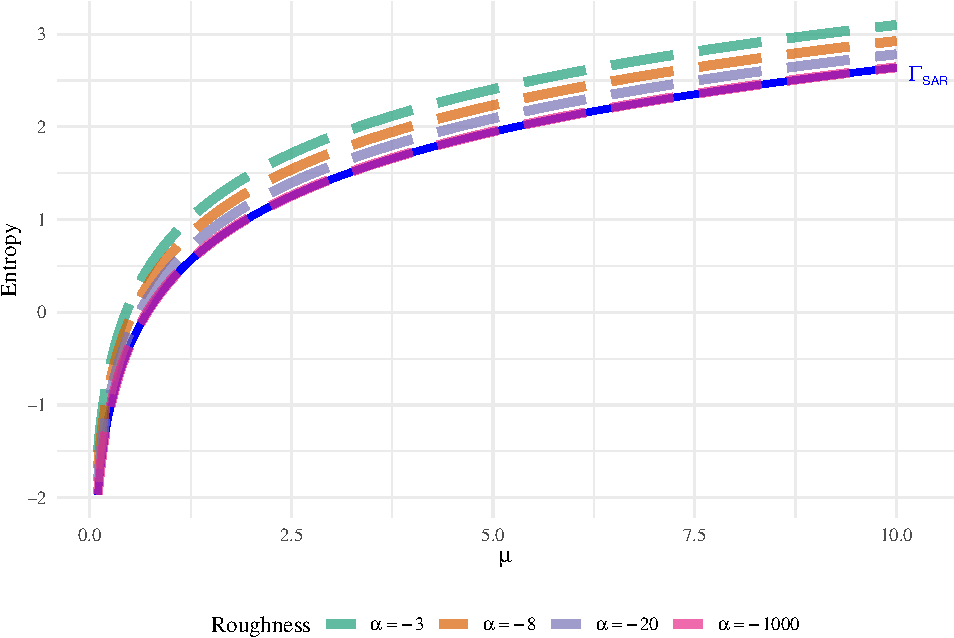
\includegraphics[scale=0.45]{./Figures/Plot_GI0_to_gamma1-1} 
        \caption*{$H_{ G_I^0}$ converges to the $H_{\Gamma_{\text{SAR}}}$, $L=8$.}
        %\label{fig:voltage}
    \end{figure}
		%\begin{block}{} 
		%\justifying
%\end{block}
\end{block}\vspace{2.8cm}
    \end{column}
\end{columns}\vspace{0.2cm}
%\metroset{block=fill}
      %\begin{exampleblock}{Objetive}
       
      %\end{exampleblock}

\end{frame} 
%----------------------------------------------------------------------------------------

\begin{frame} \frametitle{\large{Non-parametric Entropy Estimation Approach}}

 \justifying
\begin{columns}[T,onlytextwidth]
    \begin{column}{.45\textwidth}
			\begin{block}{}\justifying
 %Non-parametric approaches do not use $\widehat{\bm{\theta}}$ as a proxy. Instead, they rely on differences between order statistics.

Vasicek introduced an  non-parametric estimator in 1976: \begin{equation*}
\label{E:Vas}
    \alert<+>{\widehat{H}_{\text{V}}(\bm{Z})=\frac{1}{n}\sum_{i=1}^{n}\ln\left[\frac{n}{2m}\left(Z_{(i+m)}-Z_{(i-m)}\right)\right],}
    \end{equation*} where
\(Z_{(i+m)}-Z_{(i-m)}\) is the \(m\)-spacing and
\(Z_{(1)}\leq Z_{(2)}\leq\ldots\leq Z_{(n)}\) are the \textbf{order statistics.}

\pause

We consider superior adaptations:
\begin{itemize}
\item $\left[\text{Ebrahimi et al., 1994}\right]$: \(\widehat{H}_{\mathrm{E}}\).
\item  $\left[\text{Correa, 1995}\right]$: \(\widehat{H}_{\text{C}}\).
\item  $\left[\text{Al Omary, 2014}\right]$: \(\widehat{H}_{\mathrm{AO}}\).
\end{itemize}
		\end{block}
    \end{column}
		
  \pause  
\begin{column}{.48\textwidth}\vspace{-0.1cm}
%\metroset{block=fill}
\begin{exampleblock}{Enhanced Bootstrap Technique}
        \begin{align*}
\textcolor[rgb]{0,0,1}{\widetilde{H} = 2\widehat{\theta}(\bm{Z}) - \frac{1}{B}\sum_{b=1}^B \widehat{\theta}_b(\bm{Z}^{(b)})}
\end{align*} 
      \end{exampleblock}
					     \begin{block}{} \vspace{-0.8cm}
		\justifying
				\begin{figure}[H] 
         \centering
         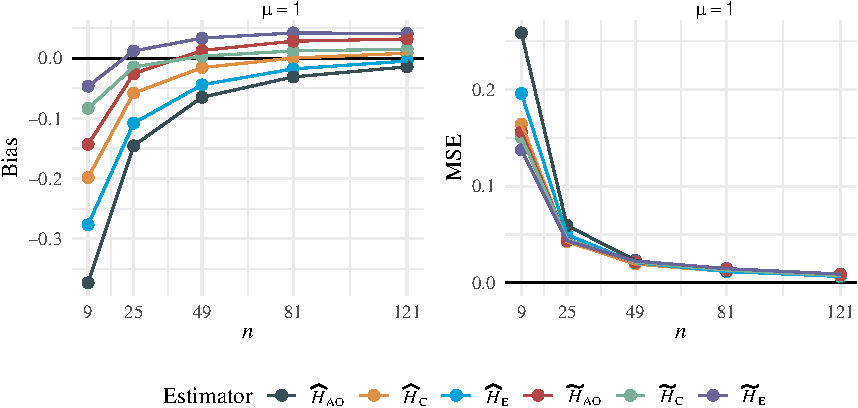
\includegraphics[scale=0.51]{./Figures/Plot_bias_mse_gi0-1} 
        \caption*{\tiny{Bias and MSE of original and bootstrap versions, $L=5$ and  $\alpha=-10$.}}
        %\label{fig:voltage}
    \end{figure}
		%\begin{block}{} 
		%\justifying
%\end{block}
\end{block}\vspace{2.8cm}
    \end{column}
\end{columns}\vspace{0.2cm}
%\metroset{block=fill}
      %\begin{exampleblock}{Objetive}
       
      %\end{exampleblock}

\end{frame} 

%----------------------------------------------------------------------------------------

\section{Hypothesis Testing}
\begin{frame} \frametitle{\large{Hypothesis Testing }}\vspace{0.1cm}

 \justifying
\begin{columns}[T,onlytextwidth]
    \begin{column}{.45\textwidth}
			\begin{block}{}\justifying
 We aim at testing the following hypotheses:

\[\textcolor[rgb]{0,0,1}{
 \begin{cases}\mathcal{H}_0: \widetilde{H}= H_{\Gamma_{\text{SAR}}}\\ 
  \mathcal{H}_1:\widetilde{H}\neq H_{\Gamma_{\text{SAR}}}.\end{cases}}
\] In other words, we verify the hypothesis that the data are
fully-developed speckle with the following \textbf{test statistic}:
\pause
\begin{equation*}
%\label{Eq:test_e}
\alert<+>{S(\bm{Z};L)= \widetilde{H}-\left[H_{\Gamma_{\text{SAR}}}(L)+\ln \widebar{\bm{Z}}\right].}
\end{equation*} The values should be around zero under the null
hypothesis and far otherwise.
		\end{block}
    \end{column}
		
\pause
\begin{column}{.52\textwidth}\vspace{-1.0cm}
  \begin{block}{} %\vspace{-0.8cm}
		\justifying
				\begin{figure}[H] 
         \centering
         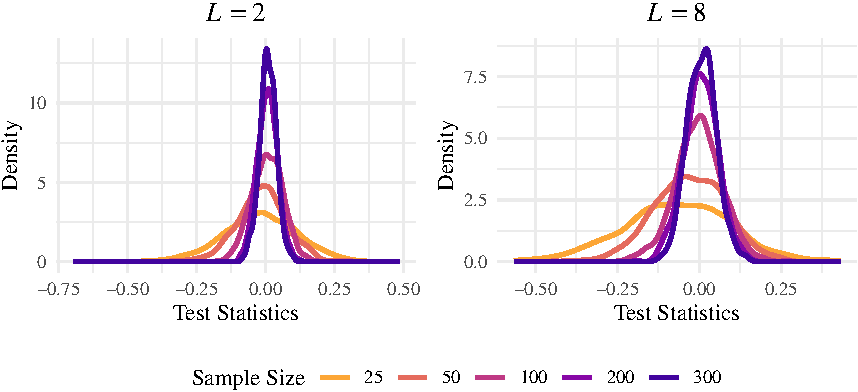
\includegraphics[scale=0.4]{./Figures/Plot_density-1} \vspace{-0.4cm}
        \caption*{\tiny{Empirical density  under the null hypothesis.}}
        %\label{fig:voltage}
    \end{figure}
\pause
\vspace{-1.0cm}
\setlength{\tabcolsep}{10pt}
\begin{table}
\colorbox{violet!10}{%
 	\resizebox{0.8\textwidth}{!}{%
  \renewcommand{\arraystretch}{1.3}
	\begin{tabular}[t]{lrrrrrrrl}
\toprule
\multicolumn{1}{c}{$\bm L$} & \multicolumn{1}{c}{$\bm n$} & \multicolumn{1}{c}{\textbf{Mean}} & \multicolumn{1}{c}{\textbf{SD}} & \multicolumn{1}{c}{\textbf{Var}}  & \multicolumn{1}{c}{\textbf{SK}} & \multicolumn{1}{c}{\textbf{EK}} & \multicolumn{1}{c}{$p$-\textbf{value}}\\
\midrule
 & $25$ & $-0.0199$ & $\phantom{-}0.1370$ & $\phantom{-}0.0188$  & $-0.3492$ & $\phantom{-}1.2320$ & $\phantom{-}0.0586$\\

 & $50$ & $-0.0145$ & $\phantom{-}0.0896$ & $\phantom{-}0.0080$  & $-0.1367$ & $\phantom{-}0.4826$ & $\phantom{-}0.0418$\\

 & $100$ & $\phantom{-}0.0064$ & $\phantom{-}0.0562$ & $\phantom{-}0.0032$  & $-0.0623$ & $-0.1617$ & $\phantom{-}0.3938$\\

 & $200$ & $\phantom{-}0.0067$ & $\phantom{-}0.0361$ & $\phantom{-}0.0013$  & $\phantom{-}0.0199$ & $-0.0305$ & $\phantom{-}0.9273$\\

\multirow{-5}{*}[2\dimexpr\aboverulesep+\belowrulesep+\cmidrulewidth]{\raggedright\arraybackslash 2} & $300$ & $\phantom{-}0.0093$ & $\phantom{-}0.0309$ & $\phantom{-}0.0010$  & $\phantom{-}0.0119$ & $\phantom{-}0.3522$ & $\phantom{-}0.1293$\\
\cmidrule{1-8}
 & $25$ & $-0.0696$ & $\phantom{-}0.1623$ & $\phantom{-}0.0264$  & $-0.1096$ & $\phantom{-}0.0158$ & $\phantom{-}0.1658$\\

 & $50$ & $-0.0301$ & $\phantom{-}0.1082$ & $\phantom{-}0.0117$  & $-0.1741$ & $\phantom{-}0.0531$ & $\phantom{-}0.2961$\\

 & $100$ & $-0.0025$ & $\phantom{-}0.0711$ & $\phantom{-}0.0051$  & $-0.0408$ & $\phantom{-}0.3446$ & $\phantom{-}0.2279$\\

 & $200$ & $\phantom{-}0.0046$ & $\phantom{-}0.0520$ & $\phantom{-}0.0027$  & $-0.0873$ & $\phantom{-}0.0466$ & $\phantom{-}0.5663$\\

\multirow{-5}{*}[2\dimexpr\aboverulesep+\belowrulesep+\cmidrulewidth]{\raggedright\arraybackslash 8} & $300$ & $\phantom{-}0.0070$ & $\phantom{-}0.0448$ & $\phantom{-}0.0020$  & $\phantom{-}0.0818$ & $\phantom{-}0.0306$ & $\phantom{-}0.5431$\\
\bottomrule
\end{tabular}}}
\caption*{\label{tab:table_stat_combined}\tiny{Descriptive analysis of $S(\bm Z; L)$ to verify the normality of the data with $L\in\left\{2, 8\right\}$ and $\mu=1$.}}
\end{table}


\end{block}\vspace{2.8cm}
    \end{column}
\end{columns}\vspace{0.2cm}
%\metroset{block=fill}
      %\begin{exampleblock}{Objetive}
       
      %\end{exampleblock}

\end{frame} 


\begin{frame} \frametitle{\large{Hypothesis Testing }}\vspace{0.5cm}

 \justifying
\begin{columns}[T,onlytextwidth]
    \begin{column}{.45\textwidth}
			\begin{block}{\small{\quad  \quad Empirical densities}}\justifying
				\begin{figure}[H] 
         \centering
         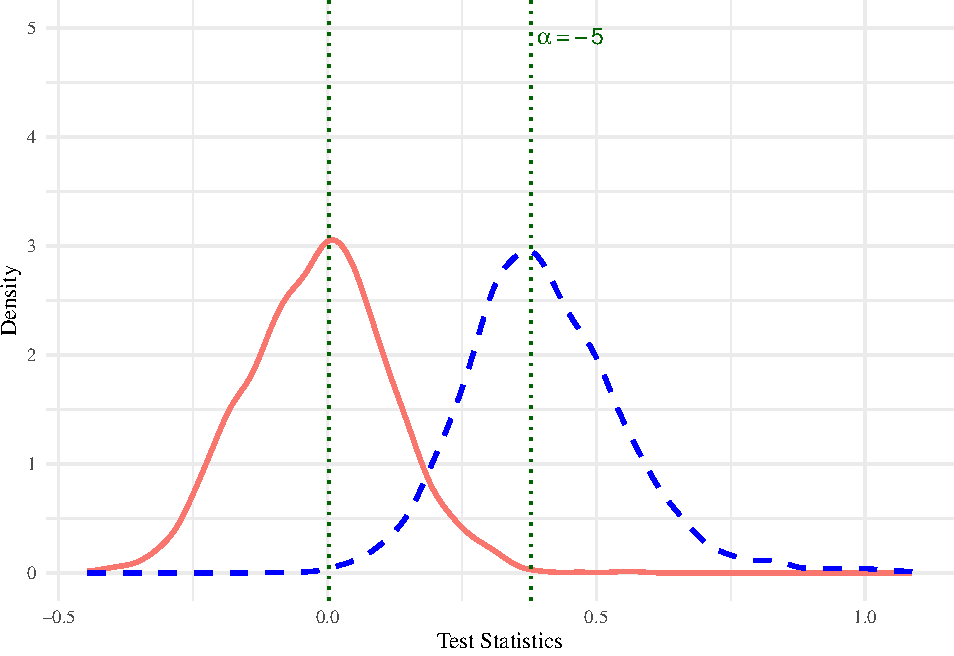
\includegraphics[scale=0.4]{./Figures/Plot_empirical_test-1} \vspace{-0.4cm}
        \caption*{\tiny{Empirical distributions under the null (centered around zero) and alternative hypotheses (e.g., $\alpha=-5$, showing a shift from zero), with $\mu=1$ and $L=8$.}}
        %\label{fig:voltage}
    \end{figure}
		\end{block}
    \end{column}
\begin{column}{.52\textwidth}%\vspace{-1.0cm}
  \begin{block}{\small{\quad \quad Size and Power of the proposed test.}} %\vspace{-0.8cm}
		\justifying
				
		%\begin{block}{} 
		%\justifying
%\end{block}
%\vspace{-1.0cm}
\setlength{\tabcolsep}{10pt}
\begin{table}
\colorbox{violet!10}{%
 	\resizebox{0.9\textwidth}{!}{%
  \renewcommand{\arraystretch}{1.3}
	\begin{tabular}[t]{lccccccc}
\toprule
\multicolumn{1}{c}{ } & \multicolumn{1}{c}{ } & \multicolumn{3}{c}{\textbf{Size}} & \multicolumn{3}{c}{\textbf{Power}} \\
\cmidrule(l{3pt}r{3pt}){3-5} \cmidrule(l{3pt}r{3pt}){6-8}
\multicolumn{1}{c}{$\bm L$} & \multicolumn{1}{c}{$\bm n$} & \multicolumn{1}{c}{$1\%$} & \multicolumn{1}{c}{$5\%$} & \multicolumn{1}{c}{$10\%$} & \multicolumn{1}{c}{$1\%$} & \multicolumn{1}{c}{$5\%$} & \multicolumn{1}{c}{$10\%$}\\
\midrule
 & 25 & $\phantom{-}0.016$ & $\phantom{-}0.071$ & $\phantom{-}0.117$ & $\phantom{-}0.564$ & $\phantom{-}0.672$ & $\phantom{-}0.745$\\

 & 50 & $\phantom{-}0.014$ & $\phantom{-}0.052$ & $\phantom{-}0.113$ & $\phantom{-}0.640$ & $\phantom{-}0.754$ & $\phantom{-}0.806$\\

 & 100 & $\phantom{-}0.010$ & $\phantom{-}0.057$ & $\phantom{-}0.103$ & $\phantom{-}0.738$ & $\phantom{-}0.838$ & $\phantom{-}0.885$\\

 & 200 & $\phantom{-}0.010$ & $\phantom{-}0.054$ & $\phantom{-}0.092$ & $\phantom{-}0.807$ & $\phantom{-}0.937$ & $\phantom{-}0.963$\\

\multirow{-5}{*}[2\dimexpr\aboverulesep+\belowrulesep+\cmidrulewidth]{\raggedright\arraybackslash 5} & 300 & $\phantom{-}0.007$ & $\phantom{-}0.058$ & $\phantom{-}0.107$ & $\phantom{-}0.850$ & $\phantom{-}0.961$ & $\phantom{-}0.988$\\
\cmidrule{1-8}
 & 25 & $\phantom{-}0.024$ & $\phantom{-}0.076$ & $\phantom{-}0.129$ & $\phantom{-}0.747$ & $\phantom{-}0.844$ & $\phantom{-}0.838$\\

 & 50 & $\phantom{-}0.015$ & $\phantom{-}0.055$ & $\phantom{-}0.104$ & $\phantom{-}0.857$ & $\phantom{-}0.919$ & $\phantom{-}0.939$\\

 & 100 & $\phantom{-}0.006$ & $\phantom{-}0.052$ & $\phantom{-}0.099$ & $\phantom{-}0.958$ & $\phantom{-}0.984$ & $\phantom{-}0.985$\\

 & 200 & $\phantom{-}0.014$ & $\phantom{-}0.043$ & $\phantom{-}0.109$ & $\phantom{-}0.989$ & $\phantom{-}0.999$ & $\phantom{-}1.000$\\

\multirow{-5}{*}[2\dimexpr\aboverulesep+\belowrulesep+\cmidrulewidth]{\raggedright\arraybackslash 8} & 300 & $\phantom{-}0.014$ & $\phantom{-}0.041$ & $\phantom{-}0.106$ & $\phantom{-}1.000$ & $\phantom{-}1.000$ & $\phantom{-}1.000$\\
\bottomrule
\end{tabular}}}
%\caption{\label{}\tiny{Size and Power of the proposed test.}}
\end{table}


\end{block}\vspace{2.8cm}
    \end{column}
\end{columns}\vspace{0.2cm}
%\metroset{block=fill}
      %\begin{exampleblock}{Objetive}
       
      %\end{exampleblock}

\end{frame} 

\section{Application to Actual Data}

\begin{frame} \frametitle{\large{Application to Actual Data }}\vspace{-0.6cm}
%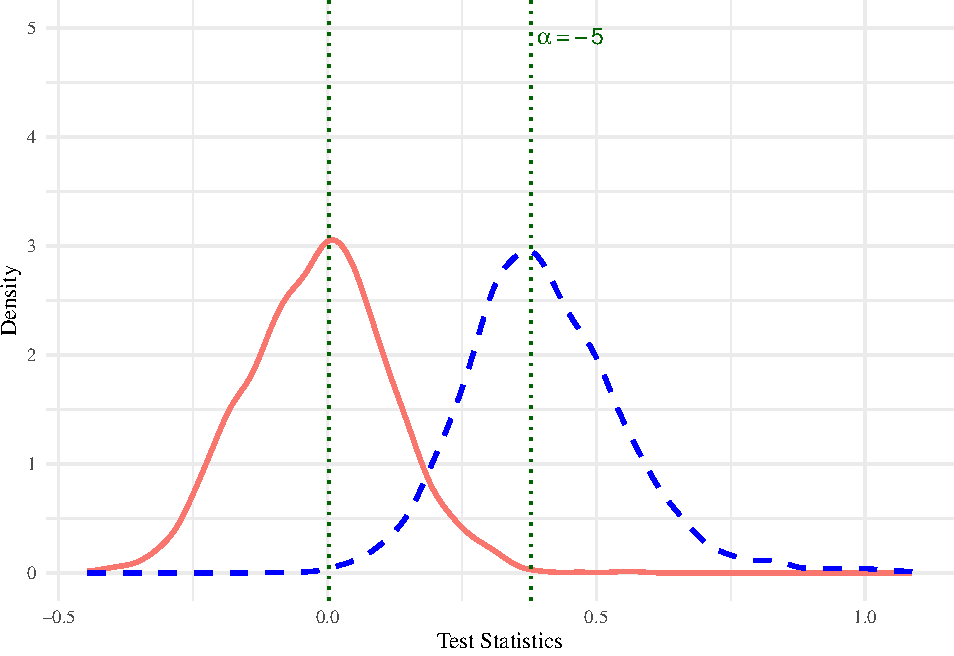
\includegraphics[scale=0.4]{./Figures/Plot_empirical_test-1} \vspace{-0.4cm}
 \justifying
\begin{columns}[T,onlytextwidth]
    \begin{column}{.99\textwidth}
			\begin{block}{}\justifying
			Images acquired by the Sentinel-1A satellite operating in the C band, with VV polarization, intensity format, and
\(L=5\) nominal looks.

Both images contain homogeneous and heterogeneous zones.
%Both images have dimensions of \(512 \times 512\) pixels and contain urban areas, agricultural fields, water and forest regions.
				\begin{figure}[H]
    \centering
    \subfloat[Flevoland ]{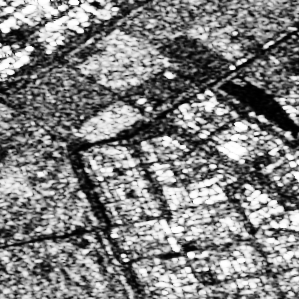
\includegraphics[width=40mm]{./Figures/Intensity} }
    \subfloat[Ottawa ]{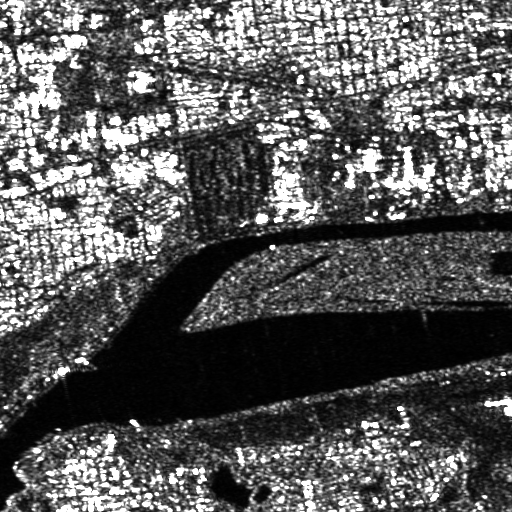
\includegraphics[width=40mm]{./Figures/Ottawa_Intensity_VV} }\vspace{-0.4cm}
    \caption*{SAR images, $300\times300$ and $512\times512$ pixels, respectively. }
    \label{fig:real_SAR_Images_coe}
\end{figure}

		\end{block}
    \end{column}

\end{columns}\vspace{0.2cm}
%\metroset{block=fill}
      %\begin{exampleblock}{Objetive}
       
      %\end{exampleblock}

\end{frame} 



\begin{frame} \frametitle{\large{Application to Actual Data }}\vspace{-0.5cm}
%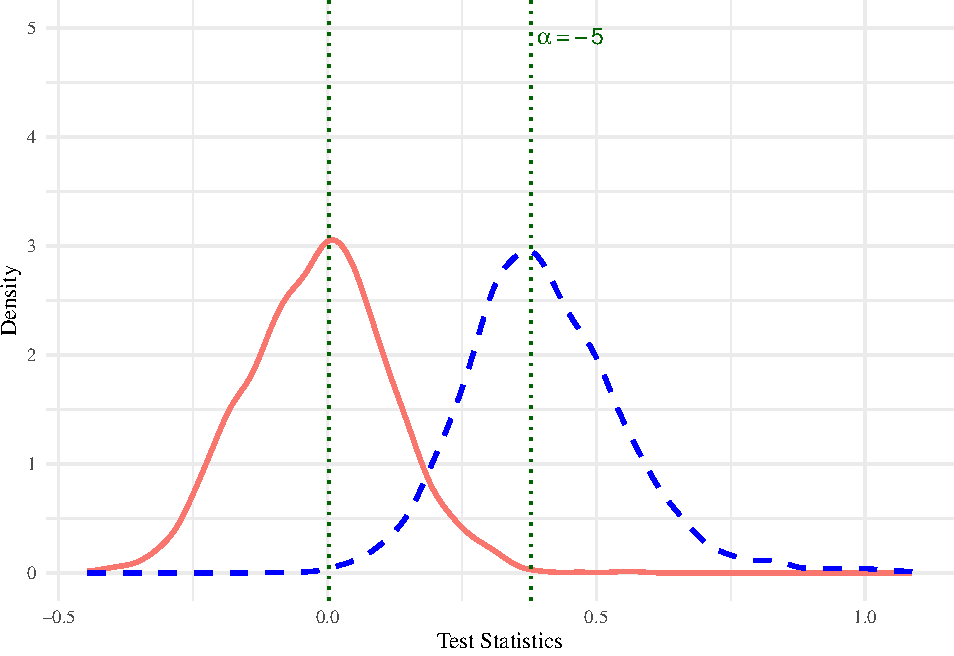
\includegraphics[scale=0.4]{./Figures/Plot_empirical_test-1} \vspace{-0.4cm}
 \justifying
\begin{columns}[T,onlytextwidth]
    \begin{column}{.99\textwidth}
			\begin{block}{}\justifying			
			The color table maps all above 0.05  into dark blue (no evidence to reject the fully-developed speckly hypothesis),
			and those below 0.05  into a gradient between blue and orange (evidence to reject the hypothesis).

		\begin{figure}[H]
    \centering
    \subfloat[Flevoland]{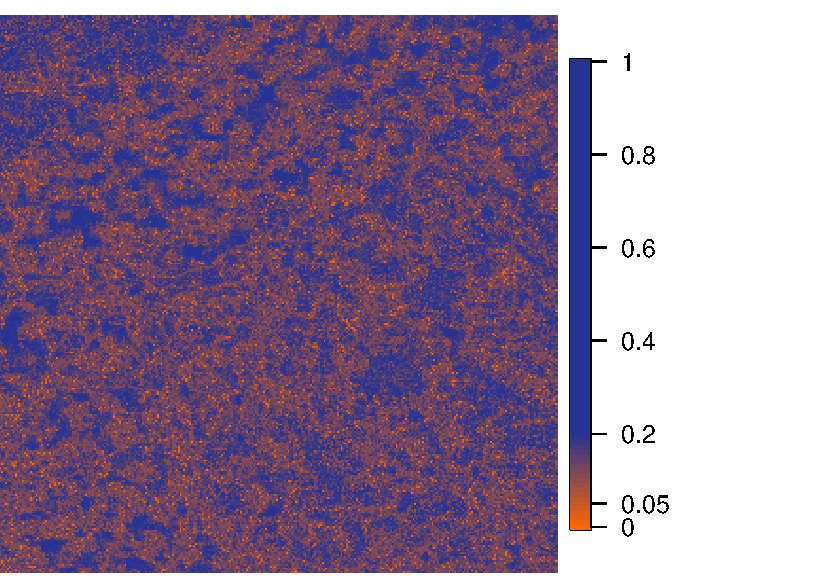
\includegraphics[width=55mm]{./Figures/Flev_300_n} }
    \subfloat[Ottawa]{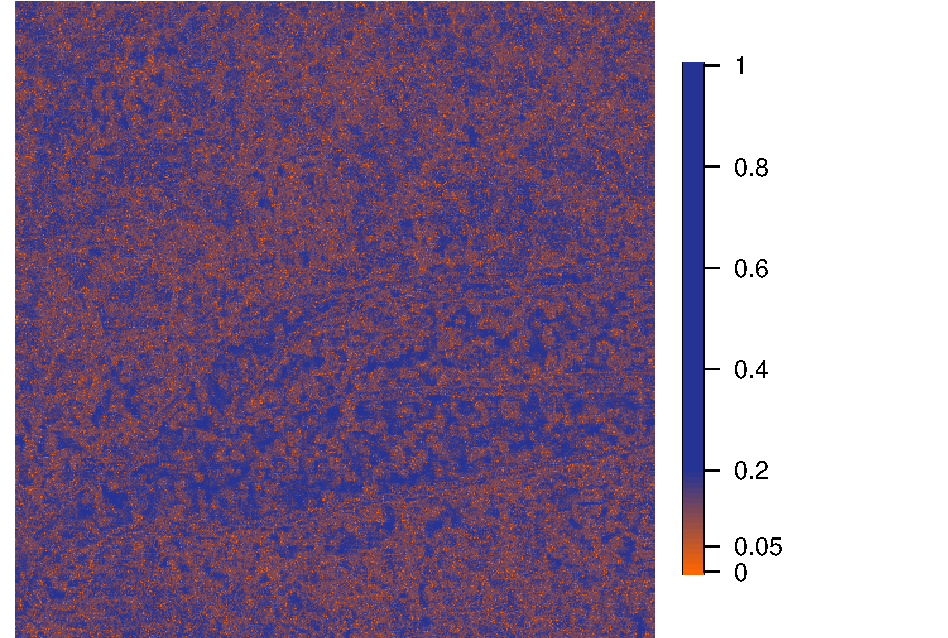
\includegraphics[width=57mm]{./Figures/Ottawa_512_f} }
    \caption*{Heatmap for a threshold of 0.05 of the $p$-values, generated after applying the proposed using 
$7\times7$ local sliding windows.}
    \label{fig:real_SAR_Images_coe}
\end{figure}

		\end{block}
    \end{column}

\end{columns}\vspace{0.2cm}
%\metroset{block=fill}
      %\begin{exampleblock}{Objetive}
       
      %\end{exampleblock}

\end{frame} 


%----------------------------------------------------

\section{Conclusions \& Future Perspectives}
\begin{frame} 
    \frametitle{\large{Conclusions \& Future Perspectives}}
    \vspace{-0.5cm}

    \justifying
    \begin{columns}[T,onlytextwidth]
        \begin{column}{.99\textwidth}
            \begin{exampleblock}{}\justifying
			
                \begin{itemize}
                    \item We proposed a testing procedure to distinguish between fully-developed speckle and heterogeneous clutter.
                    \item This tool is equipped with a test statistic based on a bootstrap-improved estimator of the Shannon entropy.
                    \item Applying the test to actual SAR data yielded promising results, effectively distinguishing different regions in the image and demonstrating the test's potential to differentiate between homogeneous and heterogeneous zones.
                \end{itemize}
                
                Currently, we are working on detecting texturelessness in SAR images. To this end, we propose novel hypothesis tests based on classical and variants of the coefficient of variation.
            \end{exampleblock}
        \end{column}
    \end{columns}
    
    \vspace{0.2cm}
\end{frame}



%---------------------------------------------------

%\begin{frame}[standout]
%  Questions?
%\end{frame}
%
%\appendix
%
%
%\begin{frame}[allowframebreaks]{Referências}
%\tiny{Algumas referências \cite{paula2021generalized,paula2017new,jammalamadaka2001topics,cordeiro2014marshall,nadarajah2012general, paula2018extended}}
%\small
%
  %\bibliography{demo}
 %\bibliographystyle{abbrv}
%
%\end{frame}
\begin{frame}
    \frametitle{\large{Q\&A}}
    \vspace{-0.5cm}
    \centering \large
    \emph{Thank you for your attention}
    
    \begin{columns}[T,onlytextwidth]
        \begin{column}{.99\textwidth}
            \begin{block}{\textbf{Contact}}
                Alejandro C. Frery\\
                alejandro.frery@vuw.ac.nz \\
                \vspace{0.4cm}
                \emph{Scan to connect}
								\vspace{0.2cm}
    \begin{picture}(0,0)
        \put(-80,-10){\makebox(0,0)[lt]{
\includegraphics[width=2.0cm]{./Figures/QRCode-WebPageVUW}}}
    \end{picture}

         \end{block}
        \end{column}
    \end{columns}
    
    
\end{frame}

\end{document}
